\documentclass[11pt]{article}
\usepackage[margin=1in]{geometry}
\usepackage{amsmath,amssymb,amsthm}
\usepackage{graphicx}
\usepackage[hidelinks]{hyperref}
\newtheorem*{theorem}{Theorem}
\newtheorem*{lemma}{Scalar mollification lemma}
\newcommand{\R}{\mathbb R}
\newcommand{\rhoM}{\rho_M}

\title{All-order compact-support modular density by one mollification}
\author{Run \texttt{fa\_banach\_001}, lane 1}
\date{12 August 2026}

\begin{document}
\maketitle

\section*{Status}

\textbf{Candidate full affirmative solution of Conjecture 1.}
The argument works for every integer $m\ge1$ under either set of hypotheses
printed in the source.  It extracts the scalar content of the source's
Lemma 12 and combines it with the ordinary $W^{m,1}$ approximate-identity
theorem.

\section*{Source conjecture}

The source is Y. Ahmida, I. Chlebicka, P. Gwiazda, and A. Youssfi,
\emph{Gossez's approximation theorems in the Musielak--Orlicz--Sobolev
spaces}, arXiv:1711.06145.  Conjecture 1 appears on PDF page 7.  It defines
\[
 V_0^mL_M(\Omega)=
 \{u\in W_0^{1,1}(\Omega)\cap W^{m,1}(\Omega):D^m u\in L_M(\Omega)\}
\]
and asks whether every $u$ in this space with compact support in $\Omega$ has
$u_k\in C_c^\infty(\Omega)$ such that all derivatives through order $m$
converge in $L^1$, while $D^m u_k$ converges modularly in $L_M$.

\begin{center}
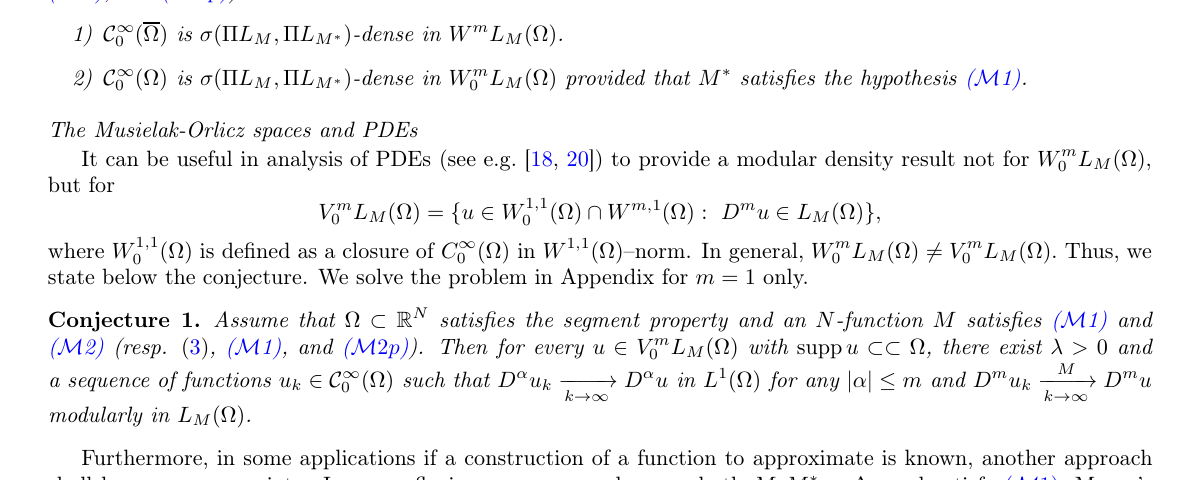
\includegraphics[width=0.98\linewidth]{figures/conjecture-crop.png}
\end{center}

Write
\[
 \rho_M(f)=\int_\Omega M(x,|f(x)|)\,dx.
\]
Modular convergence means that $\rho_M((f_k-f)/\lambda)\to0$ for some
$\lambda>0$.

\section*{The scalar observation hidden in Lemma 12}

\begin{lemma}
Assume the source's conditions $(\mathcal M1)$ and $(\mathcal M2)$; alternatively
assume (3), $(\mathcal M1)$, and $(\mathcal M2p)$.  If
$F\in L_M(\Omega)$ has compact support in $\Omega$, then
\[
 J_\varepsilon*F\longrightarrow F
 \qquad\text{modularly in }L_M(\Omega).
\]
In the alternative power-growth case, use also the resulting $F\in L^p$.
\end{lemma}

\begin{proof}
This is exactly the single-field argument in the proof of source Lemma 12,
equations (33)--(37).  By source Lemma 4, choose bounded compactly supported
$F_n$ and one $\lambda>0$ such that
$\rho_M((F_n-F)/\lambda)\to0$.  Convexity gives
\begin{align*}
 \rho_M\!\left(\frac{J_\varepsilon*F-F}{3\lambda}\right)
 &\le \frac13\rho_M\!\left(\frac{J_\varepsilon*(F-F_n)}{\lambda}\right)
   +\frac13\rho_M\!\left(\frac{J_\varepsilon*F_n-F_n}{\lambda}\right)\\
 &\qquad+\frac13\rho_M\!\left(\frac{F_n-F}{\lambda}\right).
\end{align*}
The source's mollifier estimate (Lemma 9) bounds the first term by a constant
times the third, uniformly for small $\varepsilon$; uniformity is precisely the
limit condition in $(\mathcal M2)$ (respectively $(\mathcal M2p)$).
For fixed $n$, source Lemma 5 gives translation continuity of $F_n$, and
Jensen--Fubini therefore sends the middle term to zero.  First choose $n$ and
then $\varepsilon$.  Since the modular error of $F_n$ is arbitrary, the claim
follows.  The source proof explicitly notes that the approximants need not be
derivatives, so no Sobolev structure of $F$ is used.
\end{proof}

The source states Lemma 12 for $u\in W^mL_M$:

\begin{center}
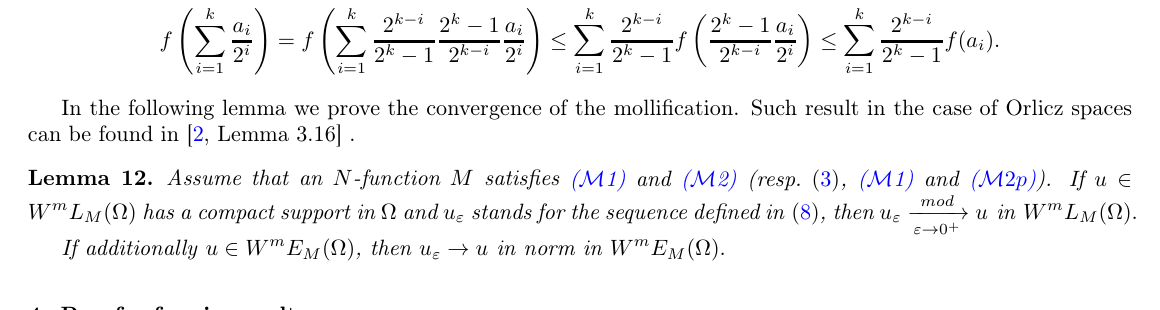
\includegraphics[width=0.96\linewidth]{figures/lemma12-crop.png}
\end{center}

Its proof applies the preceding scalar argument separately to each $D^\alpha
u$.  Retaining only one field gives the lemma above.

\section*{Full proof of Conjecture 1}

\begin{theorem}
Conjecture 1 holds for every $m\ge1$.
\end{theorem}

\begin{proof}
Let $u\in V_0^mL_M(\Omega)$ and let $K=\operatorname{supp}u\Subset\Omega$.
Extend $u$ by zero to $\R^N$.  Because $u$ vanishes on a neighborhood of
$\partial\Omega$, this zero extension belongs to $W^{m,1}(\R^N)$ and its weak
derivatives are the zero extensions of the derivatives on $\Omega$.

Set $u_\varepsilon=J_\varepsilon*u$.  If
$0<\varepsilon<\operatorname{dist}(K,\partial\Omega)$, then
$u_\varepsilon\in C_c^\infty(\Omega)$ and, for every multi-index
$|\alpha|\le m$,
\[
 D^\alpha u_\varepsilon=J_\varepsilon*D^\alpha u.
\]
Since $D^\alpha u\in L^1(\R^N)$, the standard $L^1$ approximate-identity
theorem yields
\[
 \|D^\alpha u_\varepsilon-D^\alpha u\|_{L^1(\Omega)}\longrightarrow0
 \qquad (|\alpha|\le m).
\]

For $|\alpha|=m$, the defining condition of $V_0^mL_M$ gives
$D^\alpha u\in L_M(\Omega)$, and its support lies in $K$.  The scalar
mollification lemma therefore gives
\[
 J_\varepsilon*D^\alpha u\longrightarrow D^\alpha u
 \qquad\text{modularly in }L_M(\Omega).
\]
There are only finitely many order-$m$ components.  If their number is $q$ and
their modular scales are $\lambda_\alpha$, choose
$\Lambda=q\max_\alpha\lambda_\alpha$ and use
$|D^m u_\varepsilon-D^m u|\leq\sum_{|\alpha|=m}
|D^\alpha u_\varepsilon-D^\alpha u|$ together with convexity of $M$; this
combines the componentwise statements into modular convergence of
$D^m u_\varepsilon$.

Taking any sequence $\varepsilon_k\downarrow0$ below the support distance and
putting $u_k=u_{\varepsilon_k}$ proves every conclusion of Conjecture 1.
\end{proof}

Notice that the segment property is unnecessary for this compact-interior
case; it is used elsewhere in the source to move supports that meet the
boundary.

\sloppy
\begin{thebibliography}{9}
\bibitem{ACGY}
Y. Ahmida, I. Chlebicka, P. Gwiazda, and A. Youssfi,
\emph{Gossez's approximation theorems in the Musielak--Orlicz--Sobolev
spaces}, J. Funct. Anal. 275 (2018), 1691--1714; arXiv:1711.06145.

\end{thebibliography}

\end{document}
